\documentclass[11pt]{jarticle}
\usepackage{latexsym}
\usepackage{mathrsfs}
\usepackage{amssymb}
%\usepackage{url}
%\usepackage{lscape}
\usepackage[dvipdfmx]{graphicx}
\usepackage{theorem}

%% for apple LaserWriter Series %%
%% 
\setlength{\topmargin}{-0.5in}
\setlength{\textwidth}{5.6in}
\setlength{\textheight}{8.8in}
\setlength{\oddsidemargin}{0.35in}
\setlength{\evensidemargin}{0in}

\usepackage{theorem}
\renewcommand{\baselinestretch}{1.25}
\setlength{\parskip}{0.25ex}
\renewcommand{\arraystretch}{0.85}
\begin{document}

\section{目的}

自動車のカーナビゲーションシステム,スマートフォンのロガーアプリ等で得られる地上座標の移動履歴が蓄積されたときに,
移動履歴全体あるいは部分の間で比較,検索が可能なデータとして扱うための類似性の定義を行い,
その類似性に基づく類似度計算を行うアルゴリズムを設計し,計算実験を行って適用の可能性と分野をさぐる.

\section{定義}

\subsection{位置点}
位置点は,地表上の緯度と経度の組 $(a, g) \in \mathbb{Q}^2$ (ただし $-90 \leq a \leq 90$, $-180 < g \leq 180$)である.
位置点の得られた時刻に関して真に昇順となっている列(時系列) $P = ((a_1, g_1), \ldots,(a_n,g_n))$ を軌跡 trajectory とよぶ.

現実には,
GPS では位置情報が時刻(UTC),地球上での緯度 latitude,経度 longitude の 3 つ組として得られ,ログはいくつかの一般的な形式でこれらが記録,保存される.
ここでは,列において位置点は時刻に関して真に昇順で並ぶものとして,時刻を省略する.
同様に,付加情報として標高,対地速度が情報として得られることもあるが,これらはとりあえず無視して考える.

\subsection{2 点を同一地点とみなす距離}
現実に得られる位置点の座標は,移動での変化のほか,
GPS の技術に起因する測量誤差,車線や上下線の違いなどで生じる道路の幅程度の距離の差,鉄道の線番の違いによる差など,意味的には同一地点とみなしてよいが,座標値としては異なる違いも生じる.
これに相当する距離の程度は,利用目的やデータソースなどに依存しケースバイケースになるであろうが,たとえば人の徒歩から自動車あるいは鉄道での移動について,およそ 30 秒おきに座標を得ることができるならば,数十メートルから数百メートルで考えることができる.
この同一地点とみなせる距離の最大値を $\delta > 0$ で表し,距離がこの閾値内であれば,同じ位置にあるとみなすことにする.
($\delta$ の大きさとその妥当性については,計算実験をふまえ議論する.とりあえず 50m から 500m と考えてよい.)

\subsection{2 位置点間の距離}
位置点の組 $p, q$ が与えられたとき,これらが同一地点であるかを判定,あるいは移動中の二点間の軌跡を推定するといった目的のために,
地表上での距離を求めたい.
ここでは,位置点の高度(標高)は無視できるものとして,地球を楕円体で近似し距離を求める.
ヒュベニの公式 \cite{amano-tec,GSI,Hubeny-formula-ref1,Hubeny-formula-ref2} で高次の項のみを使い $p, q$ 間の距離 $d(p,q)$ を次のように求める:
\[
d(p,q) = \sqrt{(|p_a - q_a|\cdot M)^2 + \left(|p_g - q_g|\cdot N\cos{P} \right)^2} \,,
\]
ただし緯度,経度の単位はラジアン rad であり,$P = \frac{p_a+q_a}{2}$ (緯度の平均値), $M$ は地球(楕円体)の子午線曲率半径,$N$ は同じく卯酉線曲率半径で,
地球の赤道半径 $R_x$,極半径 $R_y$,第1離心率 $e=\sqrt{\frac{R_x^2 - R_y^2}{R_x^2}}$ から,$W = \sqrt{1 - (w^2 \cdot \sin P)^2}$ とおくと
\begin{eqnarray*}
M &=& \frac{Rx\cdot (1 - e^2)}{W^3} \,, \\
N &=& \frac{Rx}{W}
\end{eqnarray*}
である.

\subsection{位置点と2点間の距離}

二つの移動履歴を表す一点列が,座標を同程度かつ十分高い頻度で記録されていない場合,
移動の軌跡はほぼ一致しても,座標点は一致しないことになる.
一方で,履歴中の位置点の間の距離が広ければ,前後する二点間の軌跡を直線として推定するのは乱暴ということになる.

そこで,点列 $P, Q$ がある場合に,
\begin{itemize}
\item[(1)] $P$ の位置点 $p_i$ と $Q$ の位置点 $q_j$ が同一視できる $d(p_i, q_j) \leq \delta$ か,
\item[(2)] $P$ の位置点 $p_i$ と $Q$ の連続する 2 つの位置点 $q_{j-1}, q_j$ を結ぶ線分との距離 $d(p_i, q_{j-1}, q_j)$ の距離が $\delta$ 以内,
\item[(3)] (2) における $P$ と $Q$ が逆,
\end{itemize}
であるときに,それぞれ一致度 $1$, $\frac{1}{2}$ と評価し,
$P$ と $Q$ の間で一致度の総和を最大化する添え字の組をもとめ,その最大値を $P, Q$ の類似度とする.
\begin{figure}[h]
\centering
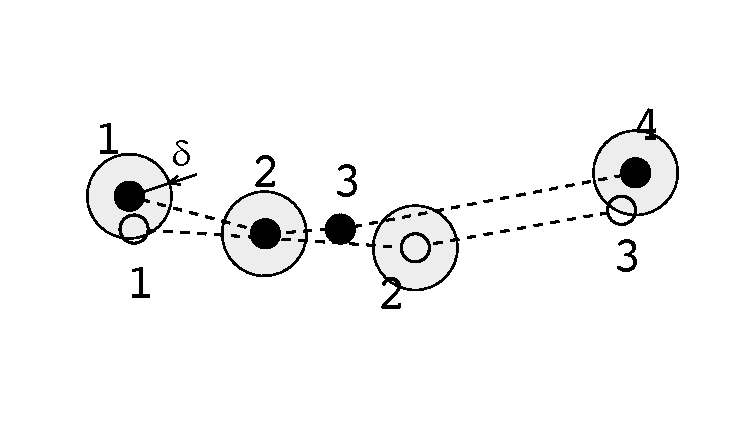
\includegraphics[scale=0.5]{matching.pdf}
%\caption{$G_1$}\label{fig:g_1}
\end{figure}

便宜的に,点列 $P=(p_1, \ldots, p_m)$ の位置点の添え字を正整数 $1 \leq i \leq m$ と $0$ または $1$ の組
$i \in \{1,\ldots, m\} \times \{0,1\}$ に拡張し,$p_{i,0}$ を位置点 $p_i$,そして $p_{i,1}$ を二点 $p_i, p_{i+1}$ の間の線分を表すとする.
ただし,列の最後の点 $p_m$ の添え字には線分を表す添え字 $(m,1)$ はないものとする.



真に増加する長さ $k \leq \min(m, n)$ の $P$ の添え字の列 $\phi_1, \ldots, \phi_k$,
すなわち $\phi_i = (\phi_i(1), \phi_i(2))$ と $\phi_{i+1} = (\phi_{i+1}(1), \phi_{i+1}(2))$ について $\phi_i(1) < \phi_{i+1}(1)$ または $\phi_i(1) = \phi_{i+1}(1)$ かつ $\phi_i(2) < \phi_{i+1}(2)$ 
 と,同じく $Q$ の添え字の列 $\psi_1, \ldots, \psi_k$ の列
を添え字の順に組にした列 $((\phi_1,\psi_1), \ldots ,(\phi_k,\psi_k))$ 
が
〜であるとき,これを位置点列 $P$ と $Q$ の共通部分列であるという.


\newpage

ある整数列(あるいは有限アルファベット上の文字列)$q = (q_1, q_2, \ldots, q_n)$ と列 $s = (s_1, \ldots, s_m)$ (ただし $m \leq n$)について,真に昇順である添え字の列 $i(1) < i(2) < \cdots < i(m)$ で $q_{i(1)} = s_1, q_{i(2)} = s_2, \ldots, q_{i(m)} = s_m$ を満たすものがあるとき,
$s$ は $q$ の部分列 subsequence であるという.

文字列の連続した一部である部分文字列 substring と異なり,部分列は列中の要素の間が(添え字の数字が)飛んでいてもよい.

\begin{example}
$q = (134, 135, 136, 135, 134, 132, 137)$ のとき,$s = (134, 135, 132, 137)$ は $q$ の部分列.
\end{example}

\begin{defn}[最長共通部分列問題 longest common sub-sequence problem]
整数(あるいは有限アルファベット中の文字)の列の組 $q, r$ が与えられたとき,
$q$ の部分列かつ $r$ の部分列となる列で,最も長いもの $s$ を求める問題.
\end{defn}

\begin{defn}[2つの位置点列の最長共通部分列 (I)]
ある正の値 $\varepsilon \in \mathbb{R}^+$ について,
二つの位置点列 $q = (s_1, \ldots, s_n)$ と $r = (t_1, \ldots, t_p)$ の間の $\varepsilon$共通部分列とは,
 $q$ と $r$ の点と点の距離が $\varepsilon$ 以内の対を点が等しいとみなした最長共通部分列 longest common super sequence である.
\end{defn}

\begin{defn}[2つの位置点列の最長共通部分列 (II)]
軌跡 $q$ の位置点および位置点と次の点の間の線分からなる列
\[
\tilde{q} = (r_1, (r_1, r_2), r_2, (r_2, r_3), r_3, \ldots, r_{n-1}, (r_{n-1}, r_n), r_n)
\]
を $q$ の経路 path という.
ある正の値 $\varepsilon \in \mathbb{R}^+$ について,
二つの位置点列 $q = (s_1, \ldots, s_n)$ と $r = (t_1, \ldots, t_p)$ それぞれの経路 $\tilde{q}, \tilde{r}$ の間の $\varepsilon$共通部分列とは,
 $\tilde{q}$ と $\tilde{r}$ の (1) 点と点の距離が $\varepsilon$ 以内,または (2) 点と線分の距離が $\varepsilon$ 以内である対を等しいとみなした最長共通部分列 longest common super sequence である.
\end{defn}

\begin{example}
例をつくってみよう.
\end{example}

\begin{thebibliography}{4}

\bibitem{amano-tec}
アマノ技研ウェブページ
\newblock  {\tt https://amano-tec.com/apps/paceruler.html}

\bibitem{toriaezu}
ヒュベニの公式
\newblock {\tt http://hp.vector.co.jp/authors/VA002244/yacht/geo.htm}

\bibitem{GSI}
国土地理院ウェブページ ``測量計算(測量計算サイト/距離と方位角の計算)''
\newblock {\tt https://vldb.gsi.go.jp/sokuchi/surveycalc/main.html}

\bibitem{Hubeny-formula-ref1}
K. Hubeny: 
\newblock Weiterentwicklung der Gauss'schen Mittelbreitenformeln, Z.Vermess, {\bf 84}, 159-163, 1959.

\bibitem{Hubeny-formula-ref2}
K. Hubeny: 
\newblock
Zur Entwicklung der Gauss'schen Mittelbreitenformeln. Osterreichische Zeitschrift fur Vernessubgswesen, {\bf 42} Jahrgang (1954) Nr.1,S. 8-17

\end{thebibliography}

\end{document}
